\chapter{Wien bridge oscillator and digital electronic}
In the first part of the experience we built a wien bridge oscillator with an automatic gain control which was made possibile by the changing resistance of a tungsten light. We focused our attention on the wave's quality and the critical time of startup. The second part was about digital electronics, after we got confident with a NAND port we designed a circuit for an house alarm system.
\section{Materials}
\begin{itemize}
\item Resistors, trimmers
\item A tungsten light
\item Power supply RIGOL DP831A
\item Waveform generator RIGOL DG1032
\item Multimeter RIGOL DM3068
\item OP741
\item DM74LS244
\item DM74LS00
\end{itemize}
The resistors used were all with an uncertainty of 5\%

\section{Experimental setup}
\subsection{Wien brigde oscillator}
For building the wien bridge and have it oscillate it is needed $R_2 = 2 R_1$, for this reason we used a trimmer as $R_2$ and a resistor of $47 \Omega$ in series with the tungsten light. We set the trimmer at a resistance around twice the resistance of 47 $\Omega$ and the light. This way when we turn on the circuit, the current start flowing in the tungsten resistor increasing its resistance, thanks to the heat produced by the current, and bringing it closer to half $R_2$. This is, in theory, what is needed for the circuit to oscillate, but it can be seen in the analysis that the circuit took some time for stablizing.
\begin{figure}[H]
\centering
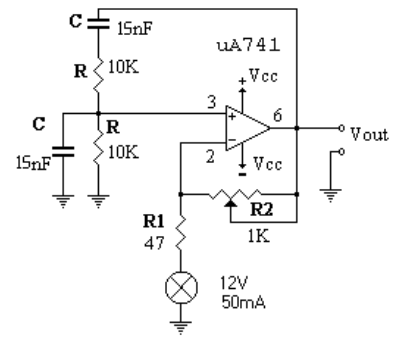
\includegraphics[width=.7\textwidth]{9/wien.png}
\caption{Wien bridge}\label{wwien}
\end{figure}
\subsection{Logic gates}
We needed to use some DM74LS00, so the first thing we did was testing it. For designing the alarm system we wrote the table of Karnaugh and minimized it.

\begin{table}[H]
\centering
\label{my-label}
\begin{tabular}{lllll}
\hline
 DW/IK & 00 & 01 & 11 & 10 \\ \hline
 00    & 0  & 0  & 0  & 1 \\
 01    & 1  & 1  & 1  & 1 \\
 11    & 1  & 1  & 1  & 1 \\ 
 10    & 1  & 1  & 1  & 1 \\ \hline
\end{tabular}\caption{D = Door, W = Window, I = Infrared, K = Key}

\end{table}

The simplified form is $Y = D + W + I\overline{C}$. The problem was that we only had NAND gates so we needed to write OR, AND and NOT with NAND. NOT is the easiest one, because you only need to connect the signal with both inputs of the NAND. AND you get it by negating the output of the NAND. For the OR gate you need to negate both input and use the two signal as input  for a NAND.


\section{Data analysis}
In the plot \ref{starting} we can see how the output oscillates a lot before stabilizing forming a sine wave (as in figure \ref{stable}) of frequency of 1122.1$\pm$1.4 Hz. The time of stabilization was around 7-8 seconds.


\begin{figure}[H]
\centering
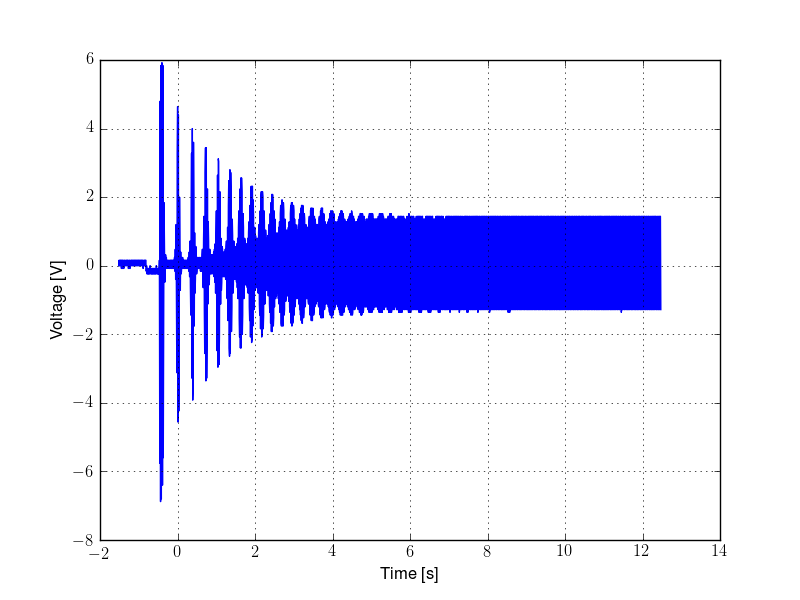
\includegraphics[width=.7\textwidth]{9/starting.png}
\caption{Starting process of the wien bridge}\label{starting}
\end{figure}

\begin{figure}[H]
\centering
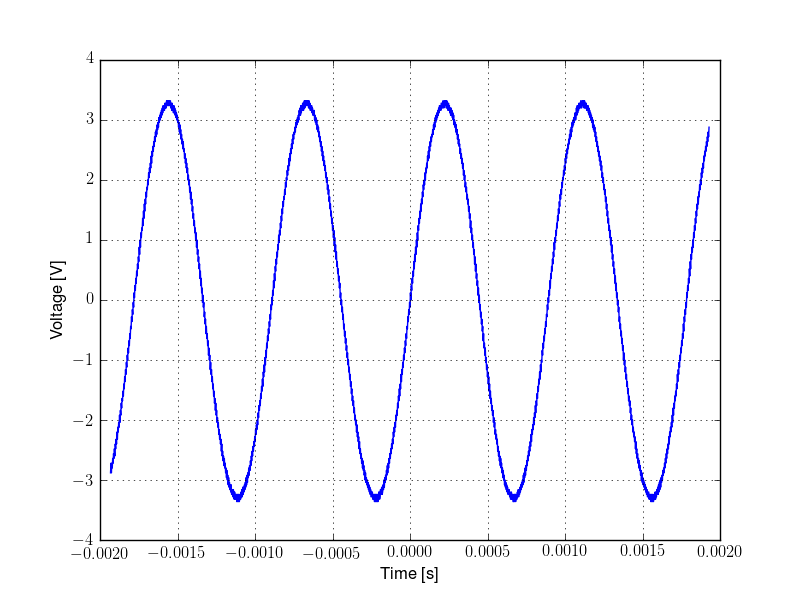
\includegraphics[width=.7\textwidth]{9/stable.png}
\caption{Stable state of the wien bridge}\label{stable}
\end{figure}

We also tested the circuit removing the by-pass capacitors and, as we can see in figure \ref{without_bypass}, the noise is too high for allowing a stable state.

\begin{figure}[H]
\centering
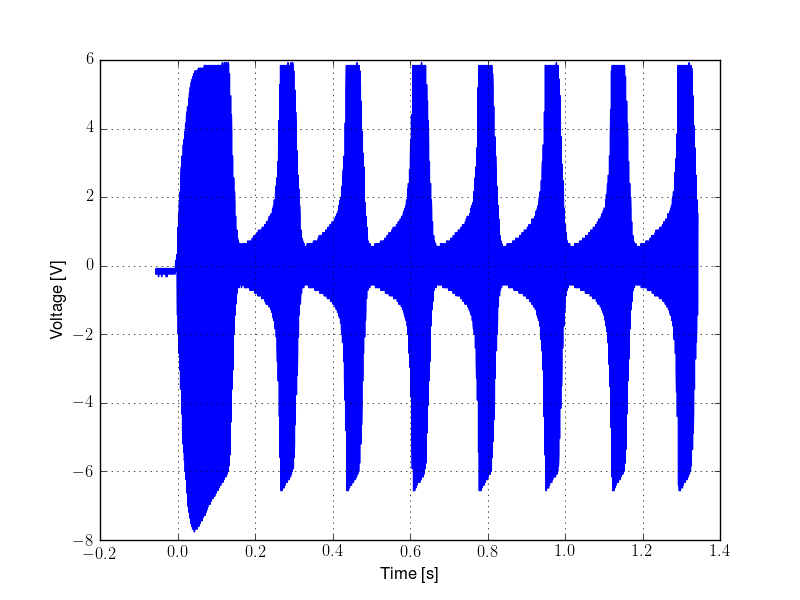
\includegraphics[width=.7\textwidth]{9/without_bypass.png}
\caption{Bridge without the by-pass capacitors}\label{without_bypass}
\end{figure}